\subsection*{1.6 Schaltkreis}
\vspace{-1mm}
\begin{minipage}{0.49\linewidth}
    \begin{footnotesize}
        \begin{center}
            \vspace{2mm}
            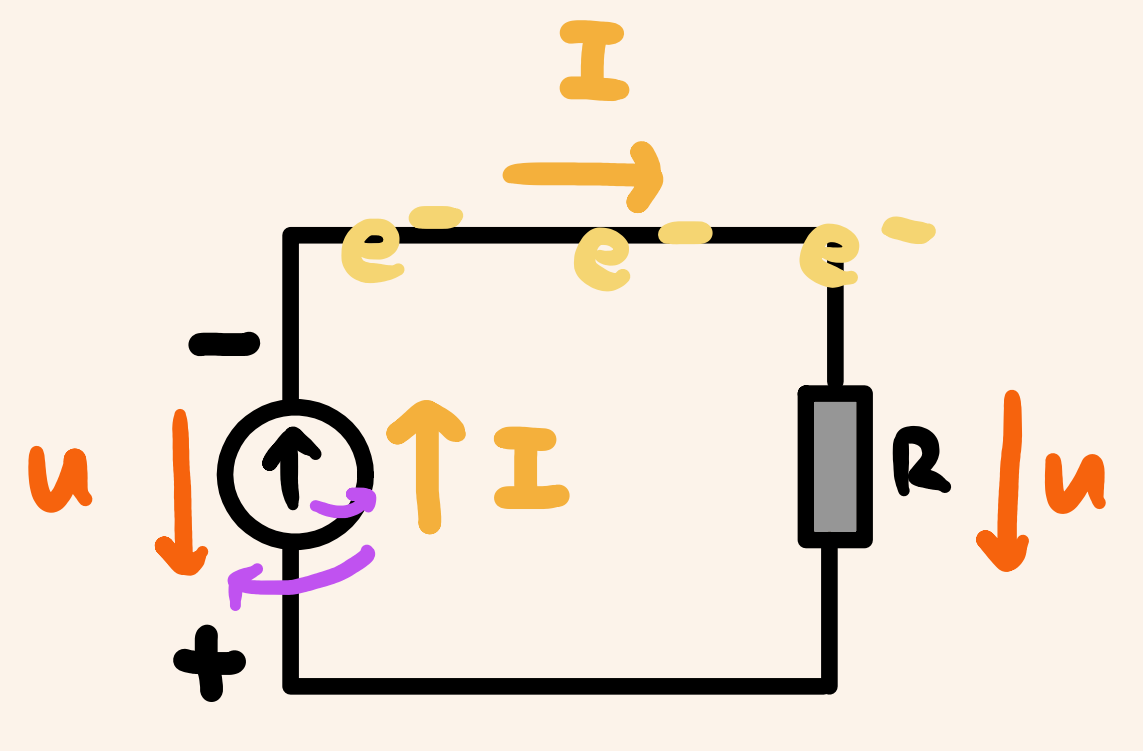
\includegraphics[width = 30mm]{src/images/schaltkreis.png}
        \end{center}
    \end{footnotesize}
\end{minipage}
\begin{minipage}{0.5\linewidth}
    \begin{scriptsize}
        \begin{center}
            \begin{align*}
                \overrightarrow{I} = &\text{ Stromrichtung}
                \\R = &\text{ Widerstand} 
                \\\overrightarrow{U} = &\text{ Richtung des Spannungsabfall}
                \\&\text{ Spannungsquelle: von mius nach plus}
                \\&\text{ Widerstand: in Stromrichtung}
            \end{align*}
        \end{center}
    \end{scriptsize}
\end{minipage}
\vspace{1mm}

    \subsubsection*{Serieschaltung}
    \vspace{-1mm}
    \begin{minipage}{0.49\linewidth}
        \begin{footnotesize}
            \begin{center}
                \vspace{2mm}
                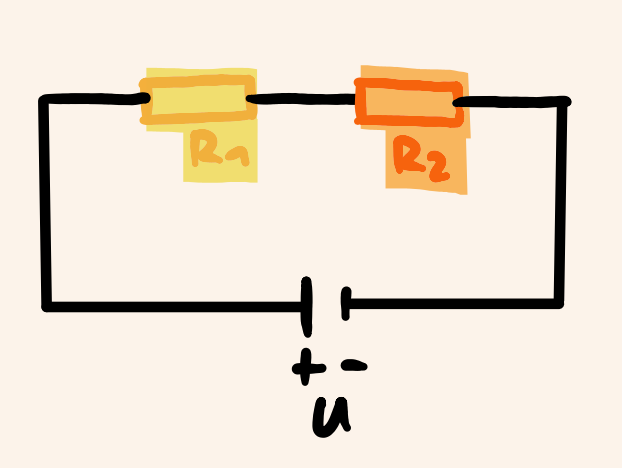
\includegraphics[width = 30mm]{src/images/serieschaltung.png}
            \end{center}
        \end{footnotesize}
    \end{minipage}
    \begin{minipage}{0.5\linewidth}
        \begin{scriptsize}
            \begin{center}
                \begin{align*}
                    R_{res} &= \sum\limits_i R_i\\
                    &= R_1 + R_2\\
                    \frac{1}{C_{res}} &= \sum\limits_i \frac{1}{C_i}
                \end{align*}
            \end{center}
        \end{scriptsize}
    \end{minipage}
    \vspace{1mm}

    \subsubsection*{Parallelschaltung}
    \vspace{-1mm}
    \begin{minipage}{0.49\linewidth}
        \begin{footnotesize}
            \begin{center}
                \vspace{2mm}
                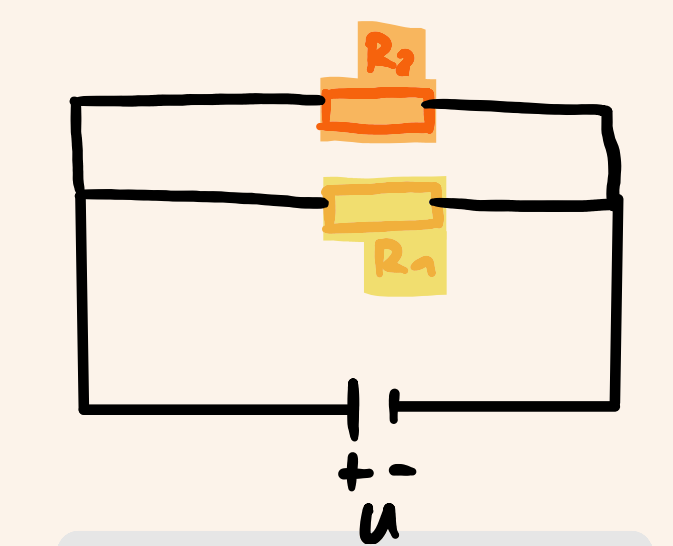
\includegraphics[width = 30mm]{src/images/parallelschaltung.png}
            \end{center}
        \end{footnotesize}
    \end{minipage}
    \begin{minipage}{0.5\linewidth}
        \begin{scriptsize}
            \begin{center}
                \begin{align*}
                    \frac{1}{R_{res}} &= \sum \frac{1}{R_i}\\
                    &= \frac{1}{R_1} +\frac{1}{R_2}\\
                    C_{res} &= \sum\limits_i C_i
                    %\\\text{Nur für zwei Widerstände:}
                    %\\R_{res} &= \frac{R_1 \cdot R_2}{R_1 + R_2}
                \end{align*}
            \end{center}
        \end{scriptsize}
    \end{minipage}
    \vspace{1mm}  